\chapter{基于样本的快速图像填充}
 \label{ch3:Inpainting}
 本章针对图像填充问题进行了研究,提出了一种基于样本的快速图像填充算法。为了使填充后的图像保持图像原有的结构信息,该算法以由粗到精的方式对图像中的缺失部分进行两次填充。在第一次填充时,首先利用离散小波变换(DWT)对输入图像进行预处理。利用DWT 的特点,提取低频子带下的低分辨率图像。利用基于样本的填充方法在此低分辨率图像上进行填充。由于低分辨率图像中的高频细节部分已经被去掉,因此第一遍填充的图像的纹理和大部分结构信息都恢复得不错,但是在包含边界的局部区域还存在着一些瑕疵。为了解决这一问题,对原图像进行第二次填充,在这次填充时只处理包含边缘结构信息的部分,使得这部分区域的结构信息能够与图像的其他部分保持连续性。为了提高图像填充的速度,提出了以动态搜索窗口结合分块结构测试的方式来搜索最佳匹配块。实验结果证明,本章所提的算法能够处理各种困难情况,达到了与目前最好的算法相近的效果。但是,本章所提的算法速度明显优于这些算法。
 \section{研究背景}
 \label{ch3:sec:background}
 图像填充问题的主要困难在于使得图像中填充后的区域在内容和结构上与周围区域保持连续性以及算法的效率。相比而言,基于样本的算法在处理结构连续性方面更好。基于样本的算法的出发点是图像中缺失部分的像素,可以以分块为单位,利用图像中已知区域中的一个或多个最佳匹配分块来填充。Criminisi等人~\cite{Criminisi04regionfilling}提出了一种基于未知区域边界法线辐射度方向计算填充优先级算法,使得未知区域以一种类似``剥洋葱皮''的顺序进行填充。虽然该算法在一些缺失部分以纹理区域为主的图像中取得了不错的效果,但是对于缺失部分包含明显图像边缘等结构信息的情况却效果不佳。如图~\ref{fig:criminisi}所示,图~\ref{fig:criminisi:1}是待处理图像,其中黑色区域为缺失部分,图~\ref{fig:criminisi:2}为文献~\inlinecite{Criminisi04regionfilling}中算法的处理结果。可以看出,填充后的三角形金字塔尖并没有恢复,填充结果存在明显的不连续情况。Xu等人~\cite{Xu:2010}指出 为了保持结构部分的连续性,应该优先填充那些包含结构信息的分块。对于图~\ref{fig:criminisi:1}中的未知区域,金字塔部分具有明显的边缘结构信息,而天空部分则为平坦的纹理区域。如果在填充时优先填充金字塔部分然后在填充天空部分,则可以避免用包含金字塔部分的分块去填充天空部分。\par
 \begin{figure}[htb]
   \centering%
   \subcaptionbox{输入图像\label{fig:criminisi:1}} %标题的长度,超过则会换行,如下一个小图。
     {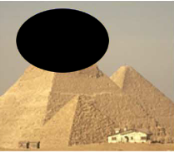
\includegraphics[width=0.3\textwidth]{fillM.png}}%
  \hspace{1em}%
   \subcaptionbox{文献~\inlinecite{Criminisi04regionfilling}算法填充结果\label{fig:criminisi:2}}
       {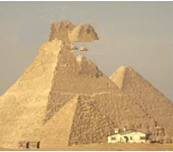
\includegraphics[width=0.3\textwidth]{fillMC.png}}
   \caption{文献~\inlinecite{Criminisi04regionfilling}算法失败例子}
   \label{fig:criminisi}
 \end{figure}
 在基于样本的图像填充算法中,由于像SSD这样的分块相似性度量指标的计算复杂度为$O(N^2)$,且搜索空间为图像全部已知区域,寻找每个缺失部分分块的最佳匹配块是一项非常耗时的工作。对于中等大小的图像,一些算法~\cite{Xu:2010}需要几分钟的时间来处理,这其中大部分时间用于分块的比较和搜索上。在实时或在线图像编辑等实际应用中,用户一般无法忍受超过1分钟的处理时间。\par
 针对以上两方面的问题,本章提出利用基于梯度结构张量(gradient structure tensor,GST)来确定填充顺序,保持填充后图像的结构连续性。为了提高算法速度,提出了一种高效的分块结构测试方法对分块进行结构相似性度量,当分块间的结构信息存在较大差距时可以直接判为不匹配分块,减少冗余的SSD 计算。同时,为了减少最佳匹配块的搜索范围,提出了一种动态搜索窗口算法,利用图像的连续性减少搜索范围。在分块匹配时,提出了用加权SSD代替SSD 进行,以改进分块间的匹配度。
 \section{相关工作}
 \label{ch3:sec:related}
针对文献~\inlinecite{Criminisi04regionfilling}算法无法处理大面积缺失区域的情况,文献~\cite{Xu:2010}提出 了一种基于分块结构稀疏性的填充算法。该算法利用分块结构稀疏性来确定填充优先级,优先填充那些结构稀疏性强的分块;在填充时通过多个候选分块的系数线性组合来计算未知区域像素值。假设$\Psi_p$是未知区域轮廓$\partial\Omega$上的一个分块,其邻域分块$\Psi_{p_{j}}$为位于以$\Psi_p$的中心点$p$为中心的窗口$N(p)$范围内的已知区域分块。$\Psi_{p_{j}}$的中心点$p_j$的集合定义为:
$$N_s(p)=\{p_j:p_j \in N(p) 且 \Psi_{p_{j}} \subset \hat{\Omega}\}$$。对于分块$\Psi_p$,其分块结构稀疏度定义为:
\begin{equation}\label{ch3:equ:sparsity}
\rho(p)=\|\vec{\omega_p}\|_{L_2}\sqrt{\frac{|N_s(p)|}{|N(p)|}}
\end{equation}

其中,$\vec{\omega_p}$为$N_s(p)$内分块之间的相似度矢量,$|\cdot|$表示所包含元素的个数。从公式~\ref{ch3:equ:sparsity}可以看出,当分块包含边缘、角点等边缘信息时,邻域内分块的相似性越差从而造成分块的结构稀疏度越大;而当邻域内主要为纹理信息时,分块之间的相似度越高使得分块结构稀疏度越小。基于分块稀疏度,文献~\cite{Xu:2010}定义分块填充优先级为:
$$P(p) = T_{[\zeta,1]}(\rho(p)) \times C(p) 。$$
其中,$C(p)$为文献~\inlinecite{Criminisi04regionfilling}算法中定义的可靠性项,$T_{[\zeta,1]}(\rho(p))$为线性变换使得$\zeta \leqslant \rho(p) \leqslant 1$, $\zeta$ 为常量0.2。在填充时,文献~\inlinecite{Xu:2010}算法利用$N$个最相似分块$\Psi_q$的线性组合来填充未知区域的像素:
$$\hat{\Psi_p}= \sum_{q=1}^{N}{ \alpha_q \Psi_q}, P(\Psi_p) = P(\hat{\Psi_{p}}) 。$$\par
文献\inlinecite{LeMeur_2011}提出利用GST来确定分块的填充优先级。与文献~\cite{Criminisi04regionfilling}中的填充优先级一样,文献文献\inlinecite{LeMeur_2011}算法中优先级由可靠性项和数据项组成,数据项定义为:
$$ D(p) = \alpha + (1-\alpha)\exp(-\frac{C}{(\lambda_1 - \lambda_2)^2})$$
其中$\lambda_1,\lambda$为图像GST的两个特征值。在填充时,文献\inlinecite{LeMeur_2011}算法利用自适应的$K$个最相似块的线性组合来计算未知区域像素。\par
文献~\inlinecite{kwokFast}提出基于DCT的快速填充算法,该算法利用DCT将图像转换到频域,通过主元分析(PCA)选择部分重要系数来进行SSD计算,从而提高效率。此外该算法还提出了一种基于梯度的预填充算法,对未知区域进行预估以方便后续的DCT计算。通过搜索数组数据结构,文献~\inlinecite{kwokFast}的算法可以在GPU上通过并行编程实现。在预填充时,假设分块内每个像素的梯度为零,那么根据前向和后向差分,在水平和垂直方向上,每个像素可以列出4个方程,使得方程数量大于未知像素数量,通过最小二乘法可以获得超定方程的最优解,使得已知区域的梯度值获得最小值。 \par
文献\inlinecite{LeMeur:2012}指出,去掉高频细节后的低分辨率图像与原图像相比要更容易完成填充,并且其填充速度与原图像相比有巨大优势。因此文献\inlinecite{LeMeur:2012}提出的填充算法首先在低分辨率下图像填充,完成后再通过超分辨率算法,将图像转换到原分辨率。\par
与上述算法不同,文献\inlinecite{Barnes:2009}提出了一种随机的图像块匹配算法,PatchMatch。该算法的目标是在两幅图像中建立每个分块的最接近邻居场(nearest-neighbor field, NNF)。在初始化阶段,该算法通过随机值来估算每个分块的NNF值$f(x,y)$。然后通过迭代过程中的随机搜索结果对匹配结果进行更新和优化。算法的主要过程如图~\ref{ch3:fig:patchmatch}所示。每次迭代时,根据从左至右,从上至下的扫描顺序进行。假设$D(\textbf{v})$为图像$A$中$(x,y)$处的分块与图像$B$中$(x,y)+ \textbf{v} $处分块之间的距离,在更新时,$f(x,y) = \arg \min\{D(f(x,y)),D(f(x-1,y)),D(f(x,y-1))\}$。通过这种传递方式, 假如$(x,y)$处有正确的匹配,那么在局部区域$R$内所有在$(x,y)$附近的邻居都将获得这一信息而找到对应的匹配块。在迭代过程中,根据随机搜索过程不断优化 $f(x,y)$ 。假设 $ \mathbf{{v_{0}}}= f(x,y)$,在随机搜索中通过测试一系列候选分块来优化$f(x,y)$。具体的搜索策略为:
$$ \mathbf{u_i} = \mathbf{v_0} + w\alpha^{i}\mathbf{R_{i}}$$
其中$\mathbf{R_{i}}$为$[-1,1] \times [-1,1]$内均匀分布的随机值,$w$为搜索半径,$\alpha$为固定值。搜索过程中检查$i=0,1,2,\ldots$直到$w\alpha^i$小于1个像素为止。通过4到5次迭代后,PatchMatch算法可以得到较准确的NNF,并且该算法还可以通过并行化编程在GPU上实现。

 \begin{figure}[htb]
  \centering%
  \subcaptionbox{初始化\label{fig:sub:pm1}} %标题的长度,超过则会换行,如下一个小图。
    {\includegraphics[width=0.25\textwidth]{ch3/pm1.png}}%
 \hspace{1em}%
  \subcaptionbox{邻域传递\label{fig:sub:pm2}}
      {\includegraphics[width=0.25\textwidth]{ch3/pm2.png}}
 \hspace{1em}
  \subcaptionbox{随机搜索\label{fig:sub:pm3}}
      {\includegraphics[width=0.25\textwidth]{ch3/pm3.png}}
  \caption{PatchMatch算法示意图~\cite{Barnes:2009}}
  \label{ch3:fig:patchmatch}
\end{figure}
 \section{算法描述}
 \label{ch3:sec:algorithm}
 设输入图像\emph{I} 中包含未知区域 \(\Omega\) 已经已知区域 \(\overline{\Omega}\),本章提出的基于样本的图像填充算法的目标是通过\(\overline{\Omega}\)的信息来计算 \(\Omega\)。和其他经典的基于样本的填充算法一样,本章所提算法的主要任务是确定填充优先级以及寻找最佳匹配块。
 \subsection{基于GST的填充优先级}
 \label{sec:sub:GST}

 定义未知区域\(\Omega\) 的轮廓为 \(\partial\Omega\), 对于 \(\partial\Omega\)上的每个像素\(p\),将以\(p\)为中心的分块\(\Psi_p\)的填充优先级定义为:
 \begin{equation}
    \label{equ:chap3:order}
    P(p)=C(p)\times D(p)
 \end{equation}

 其中 \(C(p)\) 表示可靠性项\cite{Criminisi04regionfilling},具体定义为: $$C(p)=\frac{\sum_{q\in\Psi_p\bigcap\overline{\Omega}}{C(q)}}{\left\vert{\Psi_p}\right\vert},其中$$\(\left\vert.\right\vert\)  表示计算分块中的像素数. 引入\(C(p)\) 的目的在于让那些包含更多已知像素的区域获得更高的优先级。~\ref{equ:chap3:order}中\(D(p)\) 是数据项,主要评估分块中包含结构信息的情况,增加那些包含较多结构信息分块的填充优先级。Xu等人\cite{Xu:2010}和Lemeur等人\cite{LeMeur_2011}分别提出了不同的\(D(p)\) 计算方法。本章中提出了一种基于GST 的方法。由于GST可以很好的描述图像的结构信息以及梯度方向,已经被广泛运用于图像处理领域\cite{Kothe03edgeand}。 \par
  对于图像\(I\), 其GST定义为:
  $$T=\left(\begin{array}{cc}T_{11} & T_{12} \\ T_{21} &T_{22}\end{array}\right)=\left(\begin{array}{cc}\overline{I_{\sigma,x}^2} & \overline{I_{\sigma,x}I_{\sigma,y}} \\ \overline{I_{\sigma,x}I_{\sigma,y}} & \overline{I_{\sigma,y}^2}\end{array}\right),$$
  其中 \(I_{\sigma,x}\) and \(I_{\sigma,y}\)  为图像在水平方向和垂直方向上的梯度 ,\(\overline{X}\) 表示高斯核函数\(G_{\hat{\sigma}}\) 与 \(X\)的卷积. \(T\) 的特征值 \(\lambda_1\) 和 \(\lambda_2\) 可以反映图像所包含的结构信息情况。在包含较强边缘信息的区域有 \(\lambda_1>\lambda_2\approx0\) ,而在不含边缘的平坦区域则有\(\lambda_1\approx\lambda_2\approx0\)。 \( \lambda_{1,2} \) 可以通过下式计算: $$\lambda_{1,2}=\frac{1}{2}\left(T_{11}+T_{22}\pm\sqrt{\left(T_{11}-T_{22}\right)^2+4T^2_{12}}\right)$$
  其所包含结构的方向信息可以通过下式计算:
 $$\phi=\frac{1}{2}\arctan{\left(\frac{2T_{12}}{T_{11}-T_{22}}\right)}$$
 为了评估每个分块中是否包含结构信息已经结构的方向信息,LeMeur
 等人\cite{LeMeur_2011}提出计算分块中心点的GST。为了得到区域内更为准确的结构信息,本章算法提出计算分块内所有已知像素的GST,并对结果进行直方图统计。该直方图 \(H\) 以分块内包含的结构方向作为直方图分块依据,统计区域内已知像素的结构能量 \(\lambda_1\)。相比于文献\cite{LeMeur_2011}的方法,本章算法得到的是整个分块的结构信息,比文献\cite{LeMeur_2011}只计算分块中心点的GST的方法更鲁棒。在本章算法中\(H\) 的大小(直方图中Bin的数量)为12。定义分块结构能量(patch structure energe, PSE):
 $$P_e\left(p\right)=Max\left(Sum_{b\in{H\left(p\right)}}\left(b\right)\right)$$, 其中\(H\left(p\right)\) 表示结构能量直方图。 对于图像\(I\) , 公式~\ref{equ:chap3:order} 中的数据项定义为:
 $$D(p)=(1-\alpha)P_e(p)/max_{q\in{I}}(P_e(q))+\alpha,$$ 其中 \(\alpha\) 是一个线性变换因子,使得\(D(p)\in{[\alpha,1]}\)。加入\(\alpha\) 的目的是使得数据项的值接近于可靠性项值。在本章算法中,按照参考文献\cite{Xu:2010} 中的建议将\(\alpha\)设为固定值0.2。
 \subsection{加权SSD}
 \label{sec:sub:WSSD}
 为了寻找样本分块\(\Psi_p\)的最佳匹配块,Criminisi等人\cite{Criminisi04regionfilling}借助于两个分块间已知像素的SSD类评估分块间的相似性。待填充分块\(\Psi_p\)的最佳匹配块定义为
 \begin{equation}
 \label{equ:cha03:bestmatch}
 \Psi_{\hat{q}}=arg\;min_{\Psi_q\in\Phi}d(K(\Psi_p),K(\Psi_q))
 \end{equation}
 其中,\(d(.,.)\) 表示计算两个分块之间的 SSD , \(K\)表示提取分块内的已知像素的操作 , \(\Phi\)表示搜索范围。实际上,仅仅依靠分块已知区域的SSD是无法保证找到的最佳匹配快都是最合适用于填充的分块。例如,如图~\ref{cha03:fig:1} 所示,蓝色的分块为待填充分块,绿色分块为用公式~\ref{equ:cha03:bestmatch}计算得到的最佳匹配块。在图~\ref{cha03:fig:1}左边部分图像中绿色的分块中包含了栏杆,而待填充分块主要是草地;右边部分图像中绿色分块中包含了部分树枝区域,而蓝色的待填充区域主要是天空背景。假如利用绿色分块的对应像素对蓝色分块进行填充会导致将错误的结构信息填充到未知区域,造成最终的填充结果出现明显的不连续现象。在一些情况下仅靠分块已知区域的SSD 不能找到合适的最佳匹配块对缺失部分进行填充。
 \begin{figure}[!htbp]
 	\begin{center}
 			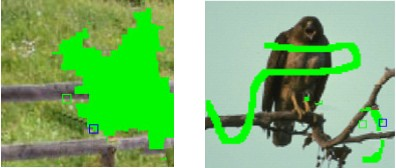
\includegraphics[width=0.8\columnwidth]{ch3/fig1.jpg}
 	\end{center}
     \caption{使用已知分块内SSD搜索造成错误匹配情况}
 	\label{cha03:fig:1}
 \end{figure}
 在文献 \inlinecite{kwokFast}中,提出了一种基于梯度的预填充方法,对待填充分块内的未知像素进行估计。基于同样的预处理方法,文献\inlinecite{jemi:2011}提出使用已知和未知区域的加权SSD (Weighted SSD,WSSD)来寻找最佳匹配块。该算法的预填充算法假设未知区域内的像素梯度值为零。基于这一假设,未知区域的像素颜色值可以通过梯度方程的最小二乘法来求解。然而,实际应用中图像较难满足梯度值为零这一假设。这这种预处理方法只考虑了分块内的局部梯度信息,最终的预处理结果并不明显。 Xu等人\cite{Xu:2010}指出,待填充分块内新填充的像素应该与周围分块保持颜色一致性和连续性。基于这一思路,本章提出了一种新的预处理方法。
 为了方便比较,本章中使用与文献\inlinecite{Xu:2010}一致的符号标识。假设 \(N(p)\) 为中心点在\(p\)的邻域窗口,集合\(N_s(p)\)定义为:
 $$N_s(p)= \left\{ p_j:p_j \in N(p)\;and\;\Psi_{p_j} \subset \overline{\Omega} \right\}.$$
 分块 \(\Psi_p\) 和\(\Psi_{p_j}\)  之间的相似性定义为:
 $$\omega_{p,p_{j}}=\frac{1}{Z(p)}exp\left(-\frac{d(K\Psi_p,K\Psi_{p_j})}{\sigma^2\left|K\Psi_p\right|}\right)$$
 其中 \(Z(p)\) 为归一化因子使得 $$\sum_{p_j\in N_s(p)}\omega_{p,p_j} = 1$$ , \(\sigma\) 为固定值5.0 \cite{Xu:2010}.\par
 令运算符\(U\) 表示从分块中提取未知像素,分块 \(\Psi_p\) 中的未知像素的预填充为
 $$U(p)=U\left(\sum_{p_j \in N_s(p)}{\omega_{p,p_j}\Psi_{p_j}}\right)$$\par
 为了寻找待填充分块的最佳匹配块, 本章提出以WSSD的方式来评估分块之间的相似性:
 \begin{equation}
 W(\Psi_p,\Psi_{p_j})=\beta\times d(K(\Psi_p),K(\Psi_{p_j}))+(1-\beta)\times d(U(\Psi_p),U(\Psi_{p_j}))
 \label{chap03:equ:wssd}
 \end{equation}
 其中加权系数 \(\beta\) 为已知区域的权值,从公式~\ref{chap03:equ:wssd}中可看出WSSD综合考虑了分块未知区域和已知区域的信息。由于未知区域是通过预填充算法估算的,因此加权系数\(\beta\)的值应该大于0.5,以使得已知部分的权值更大。在本章算法中 \(\beta\)的值建议范围为$[0.8, 0.9]$。 综上所述,分块\(\Psi_p\) 的最佳匹配块定义为:


 $$\Psi_{\hat{p}}=arg\;min_{\Psi_q \in \Phi}{W(\Psi_p,\Psi_q)}.$$


 \subsection{最佳匹配块搜索策略}
 在基于样本的图像填充算法中,主要的计算量集中在最佳匹配块的搜索中。为了提高搜索速度,文献\cite{kwokFast}提出了一种基于$K$D-tree的近似最相近邻域搜索算法,该方法主要利用高效的$K$D-tree数据结构对搜索进行加速。本章算法中,以让搜索更智能和更快为目标,提出一种智能搜索策略。由于SSD计算需要对分块每个像素进行比较,效率很低。实际上,我们人眼在搜索匹配块时并不会这样逐个像素去比较。只有当两个分块在外观上十分接近时,才可能进行这样逐个像素的比较。假如要人工完成最佳匹配块的搜索工作,人们会首先将那些明显不一致的分块放到一边不予考虑。这个预先判断和筛选的过程非常重要,本章提出利用分块结构测试的方式对分块进行测试,判断分块间结构信息是否一致。对于那些在结构上明显不一致的分块,可以直接将其排除在外,减少冗余的计算,从而加快搜索的速度。
 \subsubsection{分块结构距离测试}
 \label{sec:subsub:PST}
 在~\ref{sec:sub:GST}中,分块GST直方图被用于描述分块的结构信息。对于相似的分块,他们之间的SSD会相对较小,因此他们一定包含相似的结构信息。例如,同为不包含结构信息的两块纹理信息为主的分块,或者同为包含垂直方向边缘结构信息的分块等。对于这些相似的分块,他们的分块直方图分布也会比较相似。假如两个分块\(\Psi_p\) 、\(\Psi_q\) 的GST直方图分别为 \(H(p)\) 和 \(H(q)\),本章算法将他们之间的分块结构距离(patch structure distance, PSD)定义为\(H(p)\) 和\(H(q)\)之间的相关系数,即:

 $$PSD(p,q)=\frac{\acute{\sigma}_{pq}+c}{\acute{\sigma_p}\acute{\sigma_q}+c},$$
其中\(\acute{\sigma}_{pq}\) 为 \(H(p)\)与 \(H(q)\)之间的协方差, \(\acute{\sigma_p}\) 及 \(\acute{\sigma_q}\) 分别为 \(H(p)\) 与\(H(q)\)的标准差, \(c\) 是一个很小的常数避免出现零除以零的情况。\par
 对于待填充分块 \(p\)以及搜索窗口内的分块\(q\),当\(PSD(p,q)\)大于某门限,本章算法中门限值设置为(0.5\(\sim\)0.6), 那么认为\(p\) 和 \(q\) 在结构上存在较大差异,这也就意味着\(q\) 不可能是要寻找的最佳匹配块。这时也就没有必要再去计算他们之间的SSD。 基于此,对于候选分块\(c\),在计算 \(p\) 与 \(c\)之间的SSD时,首先测试这两者之间的PSD值是否在可接受的范围之内。对于通过PSD测试的分块,再通过SSD进一步评估分块之间的相似性,而PSD测试没有通过的分块可以直接忽略。由于\(\overline{\Omega}\) 范围内所有分块的分块GST直方图可以预先计算,且PSD 的计算复杂度远低于SSD, 引入PSD 测试可以节省很多SSD的冗余计算。\par
例如,在图~\ref{chap03:fig:PSD}中, 蓝色的分块为待填充分块,绿色矩形之内为最佳匹配块搜索范围, 红色分块为通过PSD测试的候选分块,黑色分块为本章算法搜索到的最佳匹配。从图~\ref{chap03:fig:PSD}中可以看到,由于蓝色的待填充分块包含垂直方向的边缘,所有包含水平方向边缘的分块均没有通过PSD测试。因此这些分块不可能是最佳匹配分块目标,可以直接忽略。
 \begin{figure}[!htbp]
 	\begin{center}
 			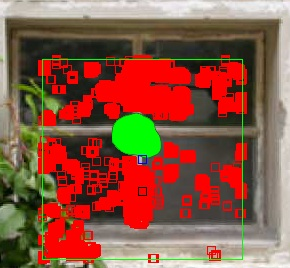
\includegraphics[width=0.6\columnwidth]{ch3/fig2.jpg}
 	\end{center}
     \caption{PSD测试示意图}
 	\label{chap03:fig:PSD}
 \end{figure}


 \subsubsection{动态搜索窗口}
 \label{sec:subsub:dynamicSearch}
 在传统的基于样本的图像填充算法中,公式~\ref{equ:cha03:bestmatch}中的 \(\Phi\)为以每个待填充区域为中心的固定窗口\cite{LeMeur_2011},或者是全部未知区域\inlinecite{Criminisi04regionfilling}。 设 \(\Psi_p\) 为中心在\(p\)处的待填充分块,考虑到图像局部范围的连续性,在\(p\)附近找到\(p\)的最佳匹配块的概率应该较大。因此定义局部窗口
 $$Win_l(p)=Win(p,sizeL)\cap \Omega,$$
 其中 \(Win(p,sizeL)\) 是大小为 \(sizeL\times sizeL\)中心点在 \( p\)的矩形窗口. \par
受到快速近似最相似邻域搜索算法PatchMatch \cite{Barnes:2009}的启发,利用图像的连续性特点,本章提出了利用邻域窗来提高搜索效率。假设 \(\Psi_q\)为 \(\Psi_p\)的相邻分块 ,即\(p\) 与\(q\)之间的距离与分块大小相等。如果 \(\Psi_q\) 已经完成了填充 ,且其最佳匹配快为 \(\hat{q}\)。那么根据图像的连续性特点,  相邻分块\(\Psi_p\)的最佳匹配块与 \(\hat{q}\)相邻的概率也会较大。 因此,定义邻域搜索窗口如下:
 $$Win_n(p)=Win(\hat{q},sizeN)\cap\Omega.$$
 当\(p\)的相邻分块中还没有一个完成填充时,\( Win_n(p)=\emptyset  \)。结合局部窗口全部搜索区域定义为:
 $$\Phi=Win_n(p)\cup Win_l(p).$$
 在图\ref{ch3:fig:3}中展示了搜索范围的一个例子。图\ref{ch3:fig:3}中,蓝色的分块为待填充分块,邻域搜索窗口和局部搜索窗口分别用红色和绿色标识,搜索到的最佳匹配块用黑色标识 。通过这种搜索方式,在图像填充过程中每个分块的最佳匹配块可以在更小的动态范围内被搜索到。因为邻域窗口的引入,局部窗口的大小可以设置得更小。在本章算法中,局部窗口和邻域窗口分别被设置为8\(\sim\)10 以及5\(\sim\)7 倍的分块大小。对于那些邻域窗口为零的分块,可以增大其局部搜索窗口的大小。\par
 \begin{figure}[!htbp]
 	\begin{center}
 			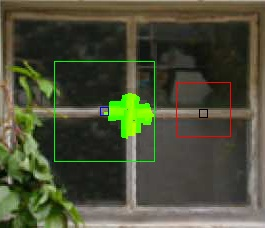
\includegraphics[width=0.6\columnwidth]{ch3/fig3.jpg}
 	\end{center}
     \caption{局部搜索窗口与邻域搜索窗口}
 	\label{ch3:fig:3}
 \end{figure}
 综上所述,本章提出的改进的基于样本的图像填充算法见算法\ref{ch3:alg:inpainting}。
 \renewcommand{\algorithmcfname}{算法}
\begin{algorithm}[!htbp]
\LinesNumbered
\KwData { 图像 \(I\),其中未知区域 \(\Omega \) ,已知区域 \(\overline{\Omega}\),  \(\Omega \) 的轮廓为 \(\partial \Omega\)}
\KwResult {填充后的图像}

   \ForEach {分块 $\Psi_q \in \overline{\Omega}$ }{
   计算分块能量直方图\(H(q)\)\;}

   \ForEach { \(\partial \Omega\)上的像素 \(p\) }{
   	 计算以$p$为中心的分块\(\Psi_p\)\ 的结构能量直方图以及PSE\;
   	 计算\(\Psi_p\) 的填充优先级 $Pri[\Psi_p]$\;}
   \While{\( \Omega \neq null\) }{
	$\Psi = \arg max_{p \in \partial \Omega}Pri[p]$\;
    按照 \ref{sec:subsub:dynamicSearch} 中的方法计算搜索窗口\(\Phi\) \;
    \ForEach {$\Psi_q$ in \(\Phi\)}{
    $d = PSD( \Psi_q,\Psi)$\;
     	\If{d < threshold}
     		{利用公式\ref{chap03:equ:wssd}计算$wd[\Psi_q]=WSSD(\Psi_q,\Psi)$\;}
     	
     	 \Else
     	 	{ $wd[\Psi_q]=MAX$\;}
     $\Psi_m = \arg min_{p \in \phi }wd[p]$ \;
     利用 \(\Psi_m\)的对应像素填充 \(\Psi\) 中的缺失部分\;
     更新\(\partial \Omega\)\;
     \ForEach{\(\partial \Omega\) 上新增像素\(n\) }
     {
     计算 \(\Psi_n\)的填充优先级$Pri[\Psi_n]$\;
     }
   }
   }
\label{ch3:alg:inpainting}
\caption{基于样本的图像填充}
\end{algorithm}

\subsection{两阶段由粗到精图像填充}
\label{sec:2.2}
对于图像填充算法来说,主要的困难在于保持输入图像中连续的结构和纹理信息以及尽可能减少图像填充过程的运算量。为了加快算法的速度,首先对输入图像进行预处理,降低其分辨率。 对输入图像进行DWT,选取低频子带图像作为输入图像的低分辨率版本。由于DWT的低频部分可以保留图像中的结构信息,因此在此低分辨率版本图像上进行填充可以保持原图中的结构信息。并且,由于低分辨率图像大小是原图像的四分之一, 使得填充速度是原图像的四倍。\par
在文献\inlinecite{LeMeur:2012}中,提出了一种与本章算法类似的两阶段填充算法,不同之处是文献\inlinecite{LeMeur:2012}算法使用超分辨率算法从填充后低分辨图像中恢复到原图像分辨率。虽然低分辨率下填充算法可以更快,但是由于随后的超分辨率算法耗时远大于填充算法,造成整个算法并没有加快速度 。与文献\inlinecite{LeMeur:2012}不同,本章算法中输入图像可以与低分辨率图像同时填充。例如,在图~\ref{ch3:fig:4}中,左边的图像\(C\)为输入图像的低分辨率版本,右边图像为相应的输入图像\(O\); 假如图像\(C\)中的分块 \(\Psi_c\) 位于 \((x,y)\), 其最佳匹配块\(\Psi_{\hat{c}}\) 的位置位于 \((i, j)\),那么图像 \(O\)中位于 \((2x, 2y)\)处的对应分块\(\Psi_o\) 可以通过 位于\((2i, 2j)\) 处的相应最佳匹配块\(\Psi_{\hat{o}}\) 来进行填充。\par
\begin{figure}[!htbp]
	\begin{center}
			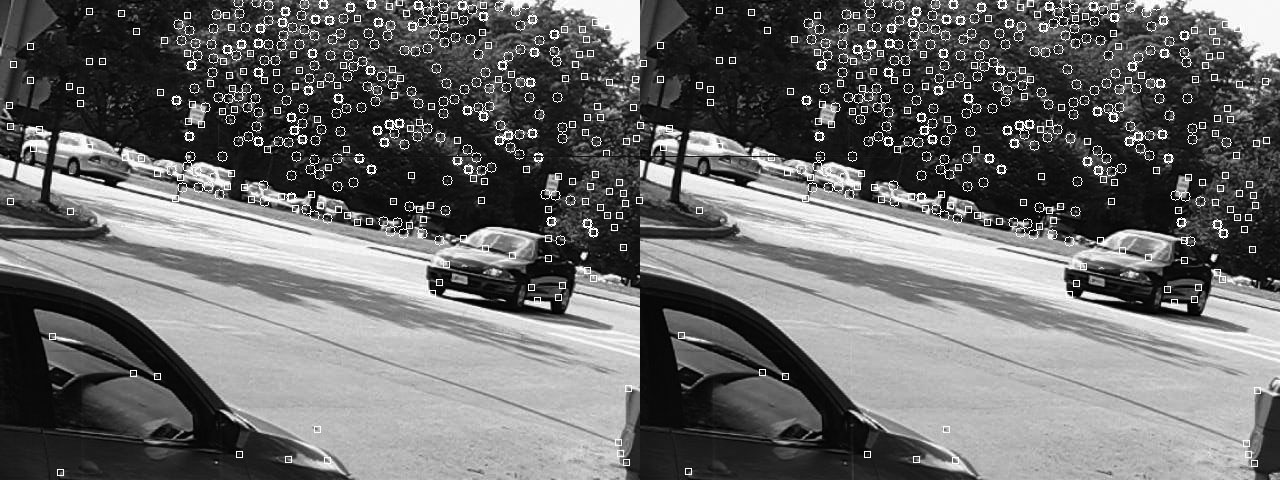
\includegraphics[width=0.6\textwidth]{ch3/fig4.jpg}
	\end{center}
    \caption{基于低分辨率版本的同步填充}
	\label{ch3:fig:4}
\end{figure}

本章提出的两阶段图像填充算法如图~\ref{ch3:fig:5}所示。在第一次填充时,低分辨率版本图像和原输入图像根据低分辨率图像填充过程进行同步填充,只取原分辨率图像的填充结果进行下一步填充。如图~\ref{ch3:fig:5}中间部分所示,第一次填充后的结果在大部分区域可以保持纹理和结构信息的连续性,但是在一些包含边缘信息的部分(见红色方框内右上角显示的放大版本)还存在一些不连续的情况。为了处理这一问题,本章算法在这些区域再进行第二阶段填充。利用PSE可以对这些包含边缘信息且存在结构不连续的区域进行定位。需要进行第二次填充的区域定义为: $$\forall p \in \Omega, P_e(p)>E_{Thres}$$。在本章算法中 \(E_{Thres}\) 设置为\(0.015 \times Max_{q\in{I}}{(P_e(p)})\)。在图~\ref{ch3:fig:5}的中间部分,可以看到需要进行第二次填充的区域小于原始区域,并且只覆盖了包含瑕疵的那部分范围。在第一次填充中,未知区域的像素已经通过预填充进行了估算,在第二次填充时则可以直接利用第一次填充的结果作为预填充结果,因此可以节省一次预填充过程。

% For one-column wide figures use
\begin{figure}[!htbp]
\begin{center}
% Use the relevant command to insert your figure file.
% For example, with the graphicx package use
  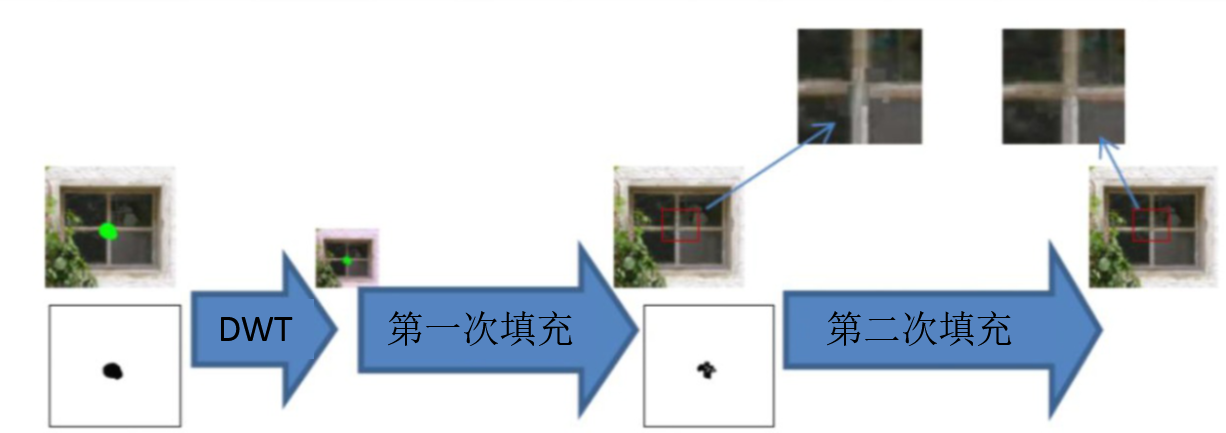
\includegraphics[width=1.0\textwidth]{ch3/flowchart.png}
% figure caption is below the figure
\end{center}
\caption{两阶段填充示意图}
\label{ch3:fig:5}       % Give a unique label
\end{figure}

 \section{实验结果与分析}
 \label{cha3:results}
为了验证本章所提算法的有效性,在大量自然图像上进行了实验。部分结果以及和现有其他算法\cite{Criminisi04regionfilling,Xu:2010}的比较如图~\ref{ch3:fig:6}所示。在实验中,第一遍填充时分块的大小设置为\(7\times7\) ,第二次填充时设置为 \(9\times9\)。和文献~\inlinecite{Xu:2010}中一样,本章所提算法中\(N_s(p)\)值设置为51。本章算法通过 C++语言实现,所有实验结果通过一台配备  Intel 2.67 GHz CPU ,512MB内存的PC上得到。\par


在图~\ref{ch3:fig:6}中,可以看到本文算法得到的填充结果可以有效的利用连续性强的结构和纹理信息对未知区域进行填充。与文献~\inlinecite{Criminisi04regionfilling}中算法相比,本文算法填充的图像效果更好,与文献~\inlinecite{Xu:2010}填充效果基本接近。\par
算法的时间比较如表~\ref{ch3:tab:timing}所示,其中所列的图像与图~\ref{ch3:fig:6}一一对应。由于计算复杂度更低,本章所提出的两阶段填充算法比文献 \inlinecite{Criminisi04regionfilling,Xu:2010}的算法更快。这主要归功于本章算法基于多分辨率的两步填充、动态搜索窗口以及PSD测试方法。
\begin{table}[htb]
\begin{center}
% table caption is above the table
\caption{算法时间比较}
\label{ch3:tab:timing}       % Give a unique label
% For LaTeX tables use
\begin{tabular}{lllll} \hline
\multicolumn{1}{c}{\multirow {2}{*}{图像}}&\multicolumn{1}{c}{\multirow {2}{*}{未知区域像素数}}& \multicolumn{3}{c}{时间(单位:秒)}\\
\cline{3-5}
\multicolumn{1}{c}{}&\multicolumn{1}{c}{}& \multicolumn{1}{c}{~\inlinecite{Criminisi04regionfilling}} &~\inlinecite{Xu:2010}&本章算法\\
\hline
\multicolumn{1}{c}{Pyramid} & \multicolumn{1}{c}{19636} & \multicolumn{1}{c}{83} &\multicolumn{1}{c}{143}& \multicolumn{1}{c}{9}\\				
\multicolumn{1}{c}{Plane} & \multicolumn{1}{c}{17914} & \multicolumn{1}{c}{82} &\multicolumn{1}{c}{130}& \multicolumn{1}{c}{10}\\				
\multicolumn{1}{c}{Riding} & \multicolumn{1}{c}{23161} & \multicolumn{1}{c}{121} &\multicolumn{1}{c}{165}& \multicolumn{1}{c}{25}\\
\multicolumn{1}{c}{Eagle} & \multicolumn{1}{c}{14837} & \multicolumn{1}{c}{84} &\multicolumn{1}{c}{108}& \multicolumn{1}{c}{17}\\
\multicolumn{1}{c}{Beach} & \multicolumn{1}{c}{6281} & \multicolumn{1}{c}{17} &\multicolumn{1}{c}{45}& \multicolumn{1}{c}{4}\\
\hline
\end{tabular}
\end{center}
\end{table}


\begin{figure}[htbp]
\begin{center}
% Use the relevant command to insert your figure file.
% For example, with the graphicx package use
  \includegraphics[width=1.0\textwidth]{ch3/fig6f.jpg}\\
  (a) 待填充图像 (b) 文献\inlinecite{Criminisi04regionfilling}算法结果  (c) 文献\inlinecite{Xu:2010}算法结果  (d) 本章算法结果
% figure caption is below the figure
\end{center}
\caption{与文献\inlinecite{Criminisi04regionfilling} 和 ~\inlinecite{Xu:2010}算法比较结果}
\label{ch3:fig:6}       % Give a unique label
\end{figure}




为了进一步验证算法的有效性,本章所提算法对文献\inlinecite{LeMeur_2011,kwokFast,LeMeur:2012}中的一些困难的例子进行了实验和对比,结果分别如图~\ref{ch3:fig:7},~\ref{ch3:fig:8},~\ref{ch3:fig:9}所示。从这些图中可以看到,由于采用了基于GST的填充优先级策略,本章算法填充后的图像可以保持原图像中那些明显的边缘部分的连续性,特别是在图中红色矩形框所标注区域。从图 ~\ref{ch3:fig:8}及图\ref{ch3:fig:9}中可以看到,本章所提算法对于那些主要由纹理构成的图像时会产生重复的纹理模式。主要原因是最佳匹配块搜寻过程中使用了基于邻域的搜索窗口。\par
\begin{figure}[!htbp]
\begin{center}
% Use the relevant command to insert your figure file.
% For example, with the graphicx package use
  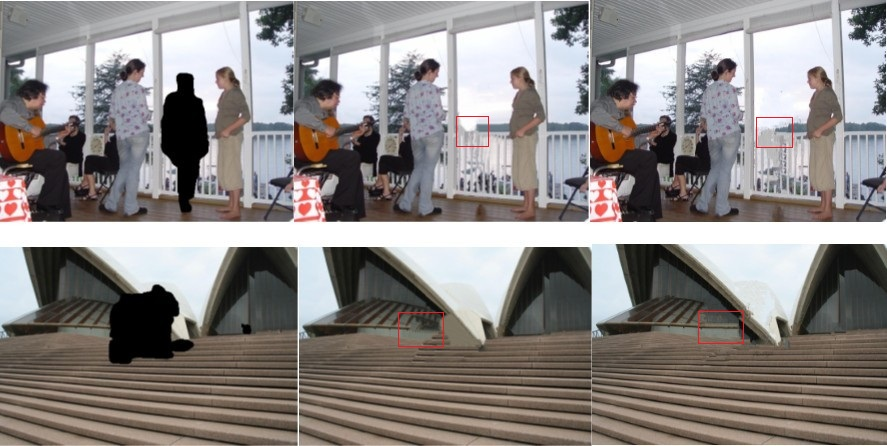
\includegraphics[width=0.8\textwidth]{ch3/fig7.jpg}\\
  (a) 待填充图像 (b) 文献\inlinecite{LeMeur_2011}算法结果    (c) 本章算法结果
% figure caption is below the figure
\end{center}
\caption{与文献~\inlinecite{LeMeur_2011}算法比较结果}
\label{ch3:fig:7}       % Give a unique label
\end{figure}
\begin{figure}[!htbp]
\begin{center}
% Use the relevant command to insert your figure file.
% For example, with the graphicx package use
  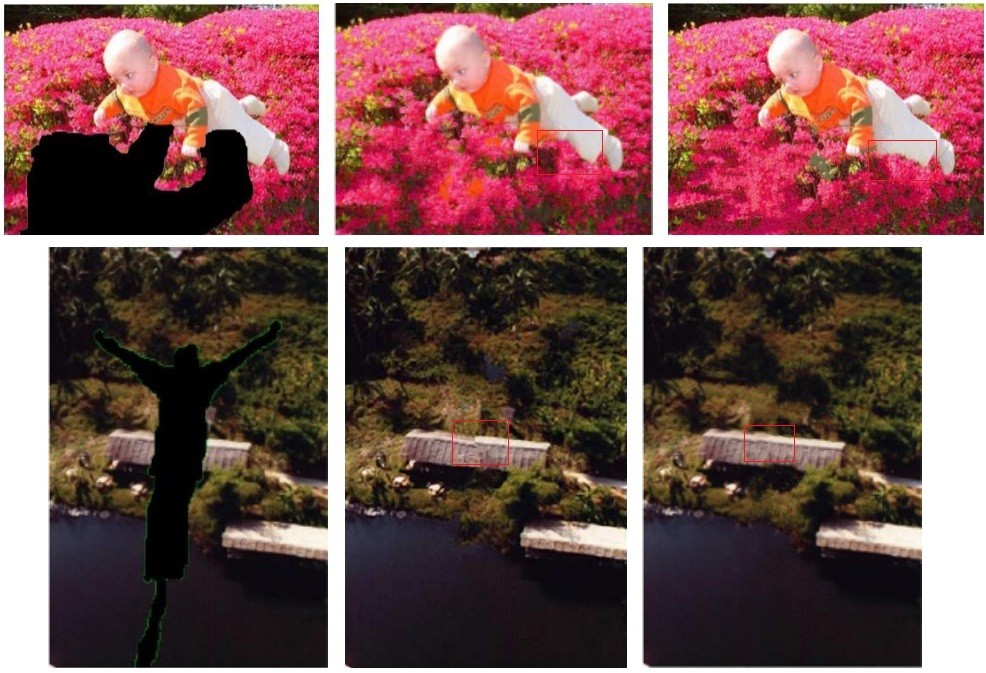
\includegraphics[width=0.8\textwidth]{ch3/fig8.jpg}
  \\
  (a) 待填充图像 (b) 文献\inlinecite{kwokFast}算法结果    (c) 本章算法结果
% figure caption is below the figure
\end{center}
\caption{与文献~\inlinecite{kwokFast}算法比较结果}
\label{ch3:fig:8}       % Give a unique label
\end{figure}

\begin{figure}[!htbp]
\begin{center}
% Use the relevant command to insert your figure file.
% For example, with the graphicx package use
  \includegraphics[width=0.8\textwidth]{ch3/fig9.jpg}
  \\
  (a) 待填充图像 (b) 文献\inlinecite{LeMeur:2012}算法结果    (c) 本章算法结果
% figure caption is below the figure
\end{center}
\caption{与文献~\inlinecite{LeMeur:2012}算法比较结果}
\label{ch3:fig:9}       % Give a unique label
\end{figure}

PatchMatch算法~\cite{Barnes:2009}已经被用于著名图像处理软件 Adobe Photoshop中的``内容感知的区域填充''功能当中。PatchMatch算法可以实现人机交互的快速填充,当待填充部分区域较小且图像中没有明显的结构信息时该算法的填充效果较好。但是,当图像中缺失部分面积过大,或图像中包含明显结构时,PatchMatch算法并不能得到满意的效果。将本章算法和PatchMatch算法针对这些困难情况进行了测试和对比,部分结果如图~\ref{ch3:fig:10} 所示,其中中间一列为PatchMatch算法填充结果,最后一列为本章算法填充结果。图~\ref{ch3:fig:10} 中的红色矩形框中显示,PatchMatch算法填充结果无法保存图像在结构上的连续性,例如在第一行和第二行图像中的栏杆部位、第三行图像中的树枝处。本章算法在这些区域的填充效果较好,可以保持栏杆等结构区域的连续性。
\begin{figure}[!htbp]
\begin{center}
% Use the relevant command to insert your figure file.
% For example, with the graphicx package use
  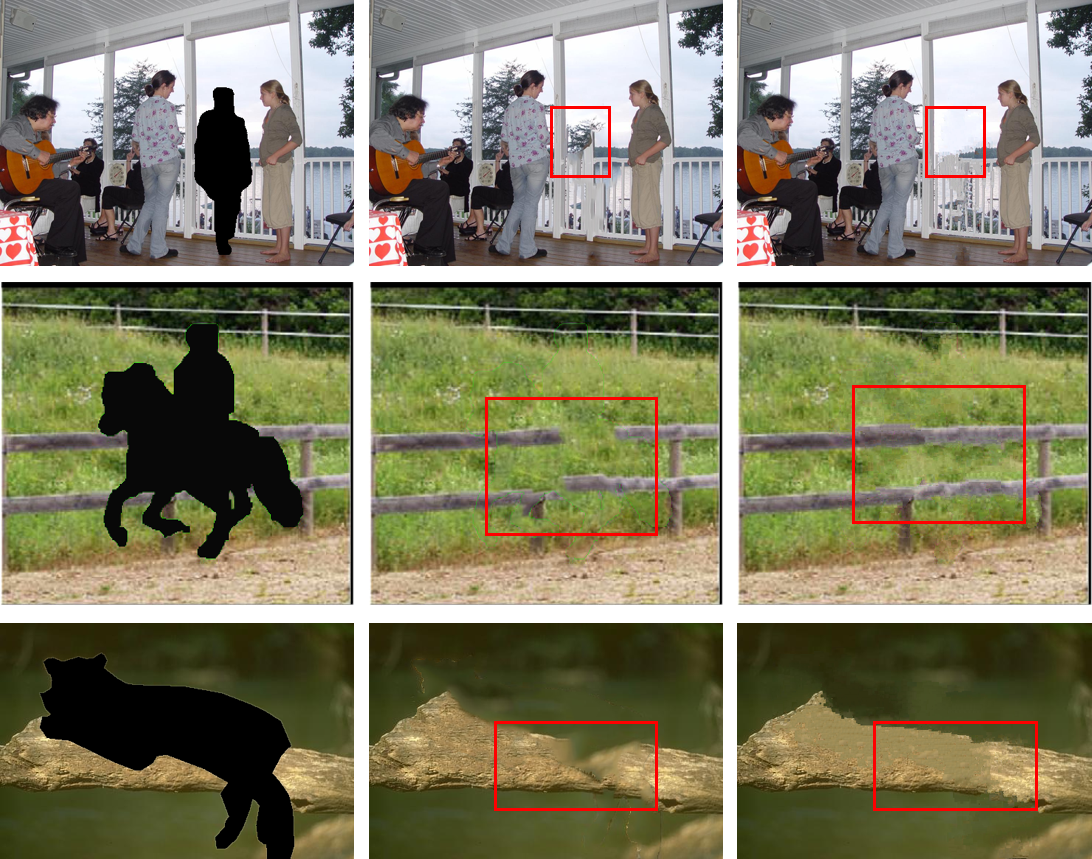
\includegraphics[width=0.8\textwidth]{ch3/VsAdobe.png}
% figure caption is below the figure
 \\
  (a) 待填充图像 (b) PatchMatch 算法\cite{Barnes:2009}结果    (c) 本章算法结果
\end{center}
\caption{与PatchMatch~\cite{Barnes:2009}算法比较结果}
\label{ch3:fig:10}       % Give a unique label
\end{figure}\par

 \section{本章小结}
 \label{cha3:conclusions}
图像填充(image inpainting)一词最早来自于艺术绘画领域,对一些早期的绘画艺术品进行保护时需要修复图画中存在的一些发黄的斑点、破损等问题。此外,图像填充技术还可以用于去掉图画中特定区域,例如在领导人合影中删除某位变节的官员等。在数字图像普及后,图像填充一般表示对数字图像进行处理,以修复其中的缺失或损坏部分的像素。图像填充技术被广泛的应用于图像处理、图像编辑以及多视图渲染等信号处理、计算机视觉和计算机图形学领域。随着数码相机、手机等移动平台的普及,日常生活中拍摄的照片经常需要进行图像填充相关的操作。\par
由于图像填充的目标是恢复未知区域的像素信息,因此在很多情况下没有正确结果来评估算法的有效性。目前一般以填充后图像的结构和纹理连续性以及图像的清晰度来评估图像填充算法。而这种连续性主要靠主观判断,很难用客观指标来评价。在保持图像中结构信息的连续性,避免产生模糊效果方面,基于样本的图像填充算法~\cite{Criminisi04regionfilling,Xu:2010}更具优势。在基于样本的图像填充算法中,需要解决的问题主要有确定填充优先级以及加快最佳匹配块的搜索速度。\par
本章对图像填充问题进行了研究,提出了一种快速的两阶段基于样本的图像填充算法。在第一阶段填充中,首先利用DWT过滤掉高频细节部分,获得低分辨率版本图像。对低分辨率图像和原始图像进行同步填充可以恢复图像中大部分区域的纹理和结构,但是在包含明显边缘部分的区域存在一些不连续的现象。在随后的第二次填充中,只对这部分有瑕疵的区域进行处理。在第二阶段填充中,使用第一阶段填充的结果作为预处理结果,作为计算\(WSSD\)的一部分。通过这种方式,已知区域的结构化和纹理信息可以很好的扩散到未知区域。本章所提出算法的主要特点有以下四点:

\begin{itemize}
 \item 基于DWT的两步填充算法可以快速得到原分辨率下的填充结果;
 \item 基于GST确定的填充优先级可以有效保证填充后图像可以很好的保持明显结构的连续性;
\item 基于图像局部和连续性特点的预填充算法更加有效和准确;
\item 使用动态搜索窗口和PSD测试,使得最佳匹配块的搜索过程更加智能和高效。
 \end{itemize}
\par
与现有其他算法相比,本章所提出的算法更加简单且易于实现。从结果效果上看,本章所提算法与当前领先的算法\cite{LeMeur:2012,Xu:2010}十分接近,但是本章算法的速度更快。在一些应用场景下,例如在线图像编辑等,需要实现实时填充,这时可以利用并行化和GPU实现\cite{kwokFast},在未来工作中,可以考虑将本章算法进行并行化。